\documentclass[a4paper, 11pt]{article}

\usepackage[utf8]{inputenc}
\usepackage[T1]{fontenc}
\usepackage[ngerman]{babel}
\usepackage[top=1.5cm, bottom=1.5cm, left=1.5cm, right=1.5cm]{geometry}
\usepackage{graphicx}
\usepackage{enumitem}

\setlength{\parindent}{0pt}
\setlist{noitemsep, topsep=3pt, leftmargin=1em}

\input{../.tmp/data}
\usepackage{fancyhdr}
\usepackage[hidelinks]{hyperref}
\pagestyle{fancy}
\fancyhf{}
\renewcommand{\headrulewidth}{0pt}
\renewcommand{\footrulewidth}{0.4pt}
\fancyfoot[L]{\footnotesize \MeinName}
\fancyfoot[R]{\footnotesize Made with \LaTeX\ \href{https://github.com/Mognus}{github.com/Mognus}}


% Abschnittsüberschrift mit Linie
\newcommand{\cvsection}[1]{%
  \vspace{0.4cm}%
  {\large\bfseries\MakeUppercase{#1}}\\[-0.1cm]%
  \rule{\linewidth}{0.4pt}%
  \vspace{0.15cm}%
}

\begin{document}

% ---- KOPFZEILE ----
\begin{minipage}[t]{0.72\textwidth}
  \vspace{0pt}
  {\Huge\bfseries \MeinName}\\[0.25cm]
  {\large \MeinTitel}
\end{minipage}
\hfill
\begin{minipage}[t]{0.22\textwidth}
  \vspace{0pt}
  \raggedleft
  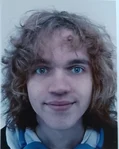
\includegraphics[width=\linewidth]{../img/magnus-profile.png}
\end{minipage}

\vspace{0.3cm}
\rule{\linewidth}{0.6pt}


% ---- ZWEISPALTIG ----
\begin{minipage}[t]{0.33\textwidth}
\vspace{0pt}

\cvsection{Kontakt}
\begin{tabular}{@{}l l}
  Tel.    & \Phone \\[2pt]
  Mail    & \small\Email \\[2pt]
  Adresse & \Address \\[2pt]
  GitHub  & \Github \\[2pt]
  Web     & \Web \\
\end{tabular}

\cvsection{Bildung}
\textbf{2022 -- 2025}\\
Andreas Gordon Schule\\
\textit{Berufsschule}

\vspace{0.3cm}

\textbf{August 2021}\\
Goetheschule Ilmenau

\cvsection{Fähigkeiten}
\begin{itemize}
  \item Python | Django | Django-REST-Framework
  \item React | Next.js | TypeScript | Zustand | Tailwind CSS | ShadCN | Headless UI | Playwright | i18n
  \item React-Native/Expo (basics)
  \item PostgreSQL | TimescaleDB | Docker | Git | GitLab CI/CD
  \item SonarQube | OWASP-Grundlagen | OAuth2/OIDC | Secure API Design | SSH Hardening
  \item Responsive Design | Component-driven UI | Design Systems | Accessibility (a11y) | Websockets
  \item Intermediate Linux Kenntnisse: Users/Groups, Filesystem, Logs, Updates/Patching, Process-/Network-Inspection; seit 4 Jahren Daily Driver (Ubuntu/KDE, danach Arch/Hyprland)
  \item KI-Tooling wie Claude Code und Codex
  \item Go | Gin | GORM | Ory | gRPC (Anfänger- bis mittlere Kenntnisse)
  \item Java (blutiger Anfänger); Interesse an JVM-basierten Sprachen, besonders Kotlin
  \item Rust (blutiger Anfänger); Grundkonzepte verstanden, bisher kaum eigene Praxis
\end{itemize}

\cvsection{Sprachen}
\begin{itemize}
  \item Deutsch: Fließend (Muttersprache)
  \item Englisch: Fließend
\end{itemize}

\end{minipage}
\hfill
\begin{minipage}[t]{0.63\textwidth}
\vspace{0pt}

\cvsection{Profil Zusammenfassung}
\begin{itemize}
  \item Junger, praxisstarker Fullstack-Webentwickler aus Thüringen mit abgeschlossener Berufsausbildung (bester Absolvent IHK Südthüringen 2025)
  \item Von August 2025 bis Januar 2026 festangestellt bei der Sielaff GmbH \& Co.\ KG
  \item Beherrscht modernes Python/Django-Backend und React/Next.js-Frontend auf Produktionsniveau, inkl.\ Docker-Deployment
  \item Suche neue Herausforderungen im Großraum Jena/Erfurt/Remote -- idealerweise Fullstack, Backend- oder DevOps-nah, aber auch für reines UI Development offen
\end{itemize}

\cvsection{Berufserfahrung}

\textbf{Sielaff Software and Service GmbH \& Co.\ KG (Ilmenau)}
\hfill \textit{Aug 2025 -- Jan 2026}\\
Fullstack Webentwickler
\begin{itemize}
  \item Weiterentwicklung, Neuentwicklung, Wartung von internen Webanwendungen im Industrie-4.0-Umfeld
  \item Fullstack-Verantwortung: Backend mit Django/DRF, Frontend mit React/Next.js
  \item Containerisierung und Deployment mit Docker, teilweise GitLab CI/CD-Pipelines
  \item Echtzeit-Kommunikation via Websockets
  \item Datenbank-Design und Optimierung
\end{itemize}

\vspace{0.35cm}

\textbf{Sielaff Software and Service GmbH \& Co.\ KG (Ilmenau)}
\hfill \textit{Ende 2022 -- Mitte 2025}\\
Ausbildung Fachinformatiker für Anwendungsentwicklung
\begin{itemize}
  \item 3-jährige duale Ausbildung mit Schwerpunkt Fullstack-Webentwicklung
  \item Entwicklung von REST-APIs, modernen Frontend-Oberflächen und internen Automatisierungs-Tools
  \item Bester Absolvent der IHK Südthüringen 2025
\end{itemize}

\end{minipage}

\end{document}
